%%%%%%%%%%%%%%%%%%%%%%%%%%%%%%%%%%%%%%%%%%%%%%%%%%%%%%%%%%%%%%%%%%%%%%%%%%%%%%%%
\begingroup
\begin{frame}{}
    \begin{block}{Applications of variational algorithms}
    \begin{itemize}
        \item Finding ground states of Hamiltonians 
        \begin{itemize}
            \item Variational Quantum Eigensolver,
            \item Quantum Adiabatic Optimization Algorithm.
        \end{itemize}
        \item Machine learning — Quantum Neural Networks, fitting model to data.
    \end{itemize}
    \end{block}
\end{frame}
\endgroup
%%%%%%%%%%%%%%%%%%%%%%%%%%%%%%%%%%%%%%%%%%%%%%%%%%%%%%%%%%%%%%%%%%%%%%%%%%%%%%%%
\begin{frame}{The idea of variational quantum computing}
    \centering
    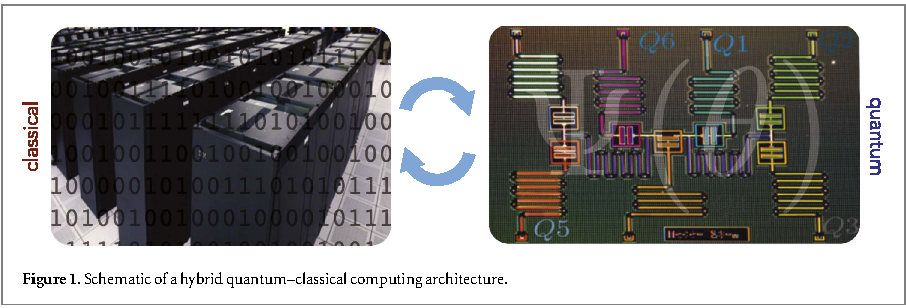
\includegraphics[page=1, width=\textwidth]{pics/vqe.pdf}
    \source{Nikolaj Moll et al 2018 \textit{Quantum Sci. Technol.} \textbf{3} 030503}
\end{frame}
%%%%%%%%%%%%%%%%%%%%%%%%%%%%%%%%%%%%%%%%%%%%%%%%%%%%%%%%%%%%%%%%%%%%%%%%%%%%%%%%
\section{Applications of Variational Quantum Eigensolvers}
\subsection{Ground state energy problem}
%%%%%%%%%%%%%%%%%%%%%%%%%%%%%%%%%%%%%%%%%%%%%%%%%%%%%%%%%%%%%%%%%%%%%%%%%%%%%%%%
\begingroup
\begin{frame}{Variational Quantum Eigensolver}
    \begin{block}{On a NISQ quantum computer}
    \begin{itemize}
        \item we can prepare $\ket{\Psi(\theta)}$ using a parametrized quantum circuit
        $\ket{\Psi(\theta)} = U(\theta_D)U(\theta_{K-1})\ldots U(\theta_1)\ket{0}$.
        \item and calculate function $E_q(\theta) = \bra{\Psi(\theta)}H_q\ket{\Psi(\theta)}$.
    \end{itemize}
    \end{block}
    \begin{block}{On a classical computer}
        \begin{itemize}
            \item we can vary parameters $\theta$.
        \end{itemize}
    \end{block}
    \begin{block}{In order to}
        \begin{itemize}
        \item find ground state energy $E_q^\text{min} = \min_\theta(\bra{\Psi(\theta)}H_q\ket{\Psi(\theta)})$.
        \end{itemize}
    \end{block}   
\end{frame}
\endgroup
%%%%%%%%%%%%%%%%%%%%%%%%%%%%%%%%%%%%%%%%%%%%%%%%%%%%%%%%%%%%%%%%%%%%%%%%%%%%%%%%
\begingroup
\begin{frame}{Variational Quantum Eigensolver}
    \begin{block}{Requirements for implementation of VQ algorithm}
        \begin{itemize}
            \item Small number of parameters $\theta$.
            \item Able to explore the problem Hilbert space.
            \item Gates $U(\theta_i)$ implemented in hardware.
        \end{itemize}
    \end{block}
    \begin{block}{Problem Hamiltonian}
    \begin{itemize}
        \item $H_q = \sum_\alpha h_\alpha P_\alpha$ --- Hamiltonian can be expressed as linear combination of 
        \item Pauli strings: $P_\alpha = \sigma_1^{\alpha_1}\otimes\sigma_2^{\alpha_2}\otimes \ldots\otimes\sigma_N^{\alpha_N}$.
        \item Where $\sigma_i^j \in \{\mathbb{1}, \sigma_i^x, \sigma_i^y, \sigma_i^z\}$.
        \item Then energy function: $E_q(\theta) = \bra{\Psi(\theta)}H_q\ket{\Psi(\theta)} = \sum_\alpha h_\alpha \bra{\Psi(\theta)}P_\alpha\ket{\Psi(\theta)}$.
    \end{itemize}
    \end{block}
\end{frame}
\endgroup
%%%%%%%%%%%%%%%%%%%%%%%%%%%%%%%%%%%%%%%%%%%%%%%%%%%%%%%%%%%%%%%%%%%%%%%%%%%%%%%%
\begingroup
\nologo
\begin{frame}{Variational quantum circuit}
    \centering
    \includegraphics[page=2, width=0.7\textwidth]{pics/vqe.pdf}
    \source{Nikolaj Moll et al 2018 \textit{Quantum Sci. Technol.} \textbf{3} 030503}
\end{frame}
\begin{frame}{Another picture of variational circuit}
    \centering
    \includegraphics[page=3, width=0.9\textwidth]{pics/vqe.pdf}
    \source{Nikolaj Moll et al 2018 \textit{Quantum Sci. Technol.} \textbf{3} 030503}
\end{frame}
\endgroup
%%%%%%%%%%%%%%%%%%%%%%%%%%%%%%%%%%%%%%%%%%%%%%%%%%%%%%%%%%%%%%%%%%%%%%%%%%%%%%%%
\begingroup
\begin{frame}{Application of VQE to quantum chemistry}
    \begin{block}{Electronic Hamiltonian in second quantization}
    \begin{itemize}
        \item Fermionic hamiltonian $H_F = \sum_{ij} t_{ij} a_i^\dagger a_j + \sum_{ijkl} t_{ij} a_i^\dagger a_k^\dagger a_l a_j$
        \item with $a_i^\dagger$ creation and $a_i$ annihilation operators.
        \item As an example of mapping of Fermionic Hamiltonian to qubits:
        \item $H_{H^2} = f_0 \mathbb{1}      \otimes \mathbb{1} + 
                        f_1 \sigma_z \otimes \sigma_z + 
                        f_2 \sigma_z \otimes \mathbb{1} + 
                        f_3 \mathbb{1}        \otimes \sigma_z + 
                        f_4 \sigma_z \otimes \sigma_z  $
        \item where $f_i$ are real coefficients dependent of the distance between atoms.
    \end{itemize}
    \end{block}
\end{frame}
\endgroup
%%%%%%%%%%%%%%%%%%%%%%%%%%%%%%%%%%%%%%%%%%%%%%%%%%%%%%%%%%%%%%%%%%%%%%%%%%%%%%%%
\subsection{Ground states of Fermionic Hamiltonians}
%%%%%%%%%%%%%%%%%%%%%%%%%%%%%%%%%%%%%%%%%%%%%%%%%%%%%%%%%%%%%%%%%%%%%%%%%%%%%%%%
\begingroup
\nologo
\begin{frame}{Finding ground state of Fermionic Hamiltonian}
    \centering
    \includegraphics[page=4, width=0.8\textwidth]{pics/vqe.pdf}
    \source{Nikolaj Moll et al 2018 \textit{Quantum Sci. Technol.} \textbf{3} 030503}
\end{frame}
\endgroup
%%%%%%%%%%%%%%%%%%%%%%%%%%%%%%%%%%%%%%%%%%%%%%%%%%%%%%%%%%%%%%%%%%%%%%%%%%%%%%%%
\subsection{Quantum Adiabatic Optimization Algorithm}
%%%%%%%%%%%%%%%%%%%%%%%%%%%%%%%%%%%%%%%%%%%%%%%%%%%%%%%%%%%%%%%%%%%%%%%%%%%%%%%%
\begingroup
\begin{frame}{Quantum Adiabatic Optimization Algorithm}
    \begin{block}{}
    \begin{itemize}
        \item Cost function $C(x)$, $x_i\in\{0,1\}$ we want to optimize.
        \item Encoding of $C$ into Hamiltonian $H_c$.
        \begin{enumerate}
            \item $x_i \rightarrow (1-z_i)/2$ with $z_i\in\{-1,1\}$,
            \item $z_i \rightarrow \sigma_i^z$
            \item $H_C = \sum_\alpha P_\alpha$
            \item where  $P_\alpha = \sigma_1^{\alpha_1}\otimes\sigma_2^{\alpha_2}\otimes \ldots\otimes\sigma_N^{\alpha_N}$ --- ``diagonal'' Pauli strings.
            \item where $\sigma_i^j \in \{\mathbb{1}, \sigma_i^z\}$.
        \end{enumerate}
        \item Mixing Hamiltonian $H_M = -\sigma_i^x$ --- transverse Hamiltonian.
        \item To find ground state of $H_C$ --- minimal value of $C(x)$:
        \item Apply $U(\beta, \gamma) = \prod_{l=1}^D e^{-i \beta_l H_M}
        e^{-i \gamma_l H_C}$ to a quantum state $\ket{\psi_0}$ and
        optimize $\gamma, \beta$ using VQE.
    \end{itemize}
    \end{block}
\end{frame}
\endgroup
%%%%%%%%%%%%%%%%%%%%%%%%%%%%%%%%%%%%%%%%%%%%%%%%%%%%%%%%%%%%%%%%%%%%%%%%%%%%%%%%
\begingroup
\subsection{Max-Cut problem and QAOA}
%%%%%%%%%%%%%%%%%%%%%%%%%%%%%%%%%%%%%%%%%%%%%%%%%%%%%%%%%%%%%%%%%%%%%%%%%%%%%%%%
\begin{frame}{Max-Cut problem}
    \begin{block}{}
    \begin{itemize}
        \item Given a graph with the edge weights $w_{ij}: w_{ij}>0, w_{ij}=w_{ji}$.
        \item Divide the graph into two disjoint subsets of vertices
        such that sum of weights between them is maximal.
        \item We want to maximize $C(x) = \sum_{ij} w_{ij} x_i(1-x_j)$, $x_i \in \{0,1\}$.
        \item $H_I=\sum_{i<j}w_{ij}(\mathbb{1}-\sigma_i^z)(\mathbb{1}+\sigma_j^z) = - \frac{1}{2} \sum_{i<j} w_{ij}\sigma_i^z\sigma_j^z+\text{const.}$
        \item Effectively: $H_C= \sum_{i<j} w_{ij}\sigma_i^z\sigma_j^z$.
    \end{itemize}
    \end{block}
\end{frame}
\endgroup
%%%%%%%%%%%%%%%%%%%%%%%%%%%%%%%%%%%%%%%%%%%%%%%%%%%%%%%%%%%%%%%%%%%%%%%%%%%%%%%%
\begin{frame}{Max-Cut using QAOA}
    \centering
    \includegraphics[page=5, width=\textwidth]{pics/vqe.pdf}
    \source{Nikolaj Moll et al 2018 \textit{Quantum Sci. Technol.} \textbf{3} 030503}
\end{frame}
%%%%%%%%%%%%%%%%%%%%%%%%%%%%%%%%%%%%%%%%%%%%%%%%%%%%%%%%%%%%%%%%%%%%%%%%%%%%%%%%
